\section{Computação Clássica} 
\label{classic_comp}
Como já mencionado anteriormente, Alan Turing – matemático inglês, cientista da computação, lógico, criptoanalista, filósofo e biólogo teórico – publicou o artigo ``On Computable Numbers with an Application to the Entscheidungs-problem'' \cite{8} em 12 de novembro de 1937, artigo que viria a constituir a teoria básica da computabilidade, que se faz presente até hoje. 

O mecanismo abstrato descrito no artigo de Turing fornece os conceitos fundamentais de computadores que outros engenheiros conceberam posteriormente. Na sua essência, uma Máquina de Turing é um dispositivo que manipula símbolos em uma tira de fita de acordo com uma tabela de regras, funcionamento que possibilitou a formalização dos conceitos de ``algoritmo'' e ``computação''. Ainda, apesar da simplicidade da Máquina de Turing, ela pode ser adaptada para simular a lógica de qualquer algoritmo de computador.

Apesar de hoje se ter a compreensão das contribuições de Alan Turing para a base da computação, os computadores clássicos são atualmente descritos como tendo a chamada arquitetura de von Neumann. No entanto acredita-se que o idealizador dessa arquitetura partiu dos modelos matemáticos desenvolvidos por Turing\cite{10}, que incluía o conceito de programa armazenado, originado a partir da construção da Máquina de Turing. Conceito, também encontrado no projeto EDVAC de von Neumann \cite{9}, que possibilita o armazenamento de instruções e dados na mesma memória, permitindo a manipulação de programas como dados, que se constitui como característica do computador clássico.  

Assim, pode-se considerar Turing como pai do computador, já que suas publicações antecedem a arquitetura de von Neumann. Ademais, tem-se que Turing foi o primeiro a explorar a idéia de uma máquina de uso geral por meio de sua noção de máquina universal – que constitui a base do computador clássico ao possibilitar o funcionamento da CPU em conjunto com a memória RAM. Ainda, tendo em vista as contribuições do matemático para a construção de uma classe importante de dispositivos de computação: o Bombe – um dispositivo eletromecânico usado pelos criptologistas britânicos para ajudar a decifrar as mensagens secretas criptografadas pela máquina alemã Enigma durante a Segunda Guerra Mundial – e posteriormente o seu design do ACE (Automatic Computing Engine), fica evidente as contribuições de Alan Turing para a invenção do computador moderno. A partir da fala de Turing abaixo, pode-se identificar o ACE como um tipo de realização física da máquina universal.

\textit{
  ``Some years ago I was researching on what might now be described as an investigation of the theoretical possibilities and limitations of digital computing machines. […] Machines such as the ACE may be regarded as practical versions of this same type of machine.'' \cite{11}
}

Por fim, entende-se que baseado na teoria da máquina de Turing, o físico e matemático John von Neumann desenvolveu uma arquitetura que consiste em uma única memória compartilhada para programas e dados; um único acesso à memória; uma unidade aritmética e uma unidade de controle de programa - ilustrado no diagrama abaixo.

\vspace{1cm}
\begin{figure}[H] \centering 
  \makebox[\textwidth][c]{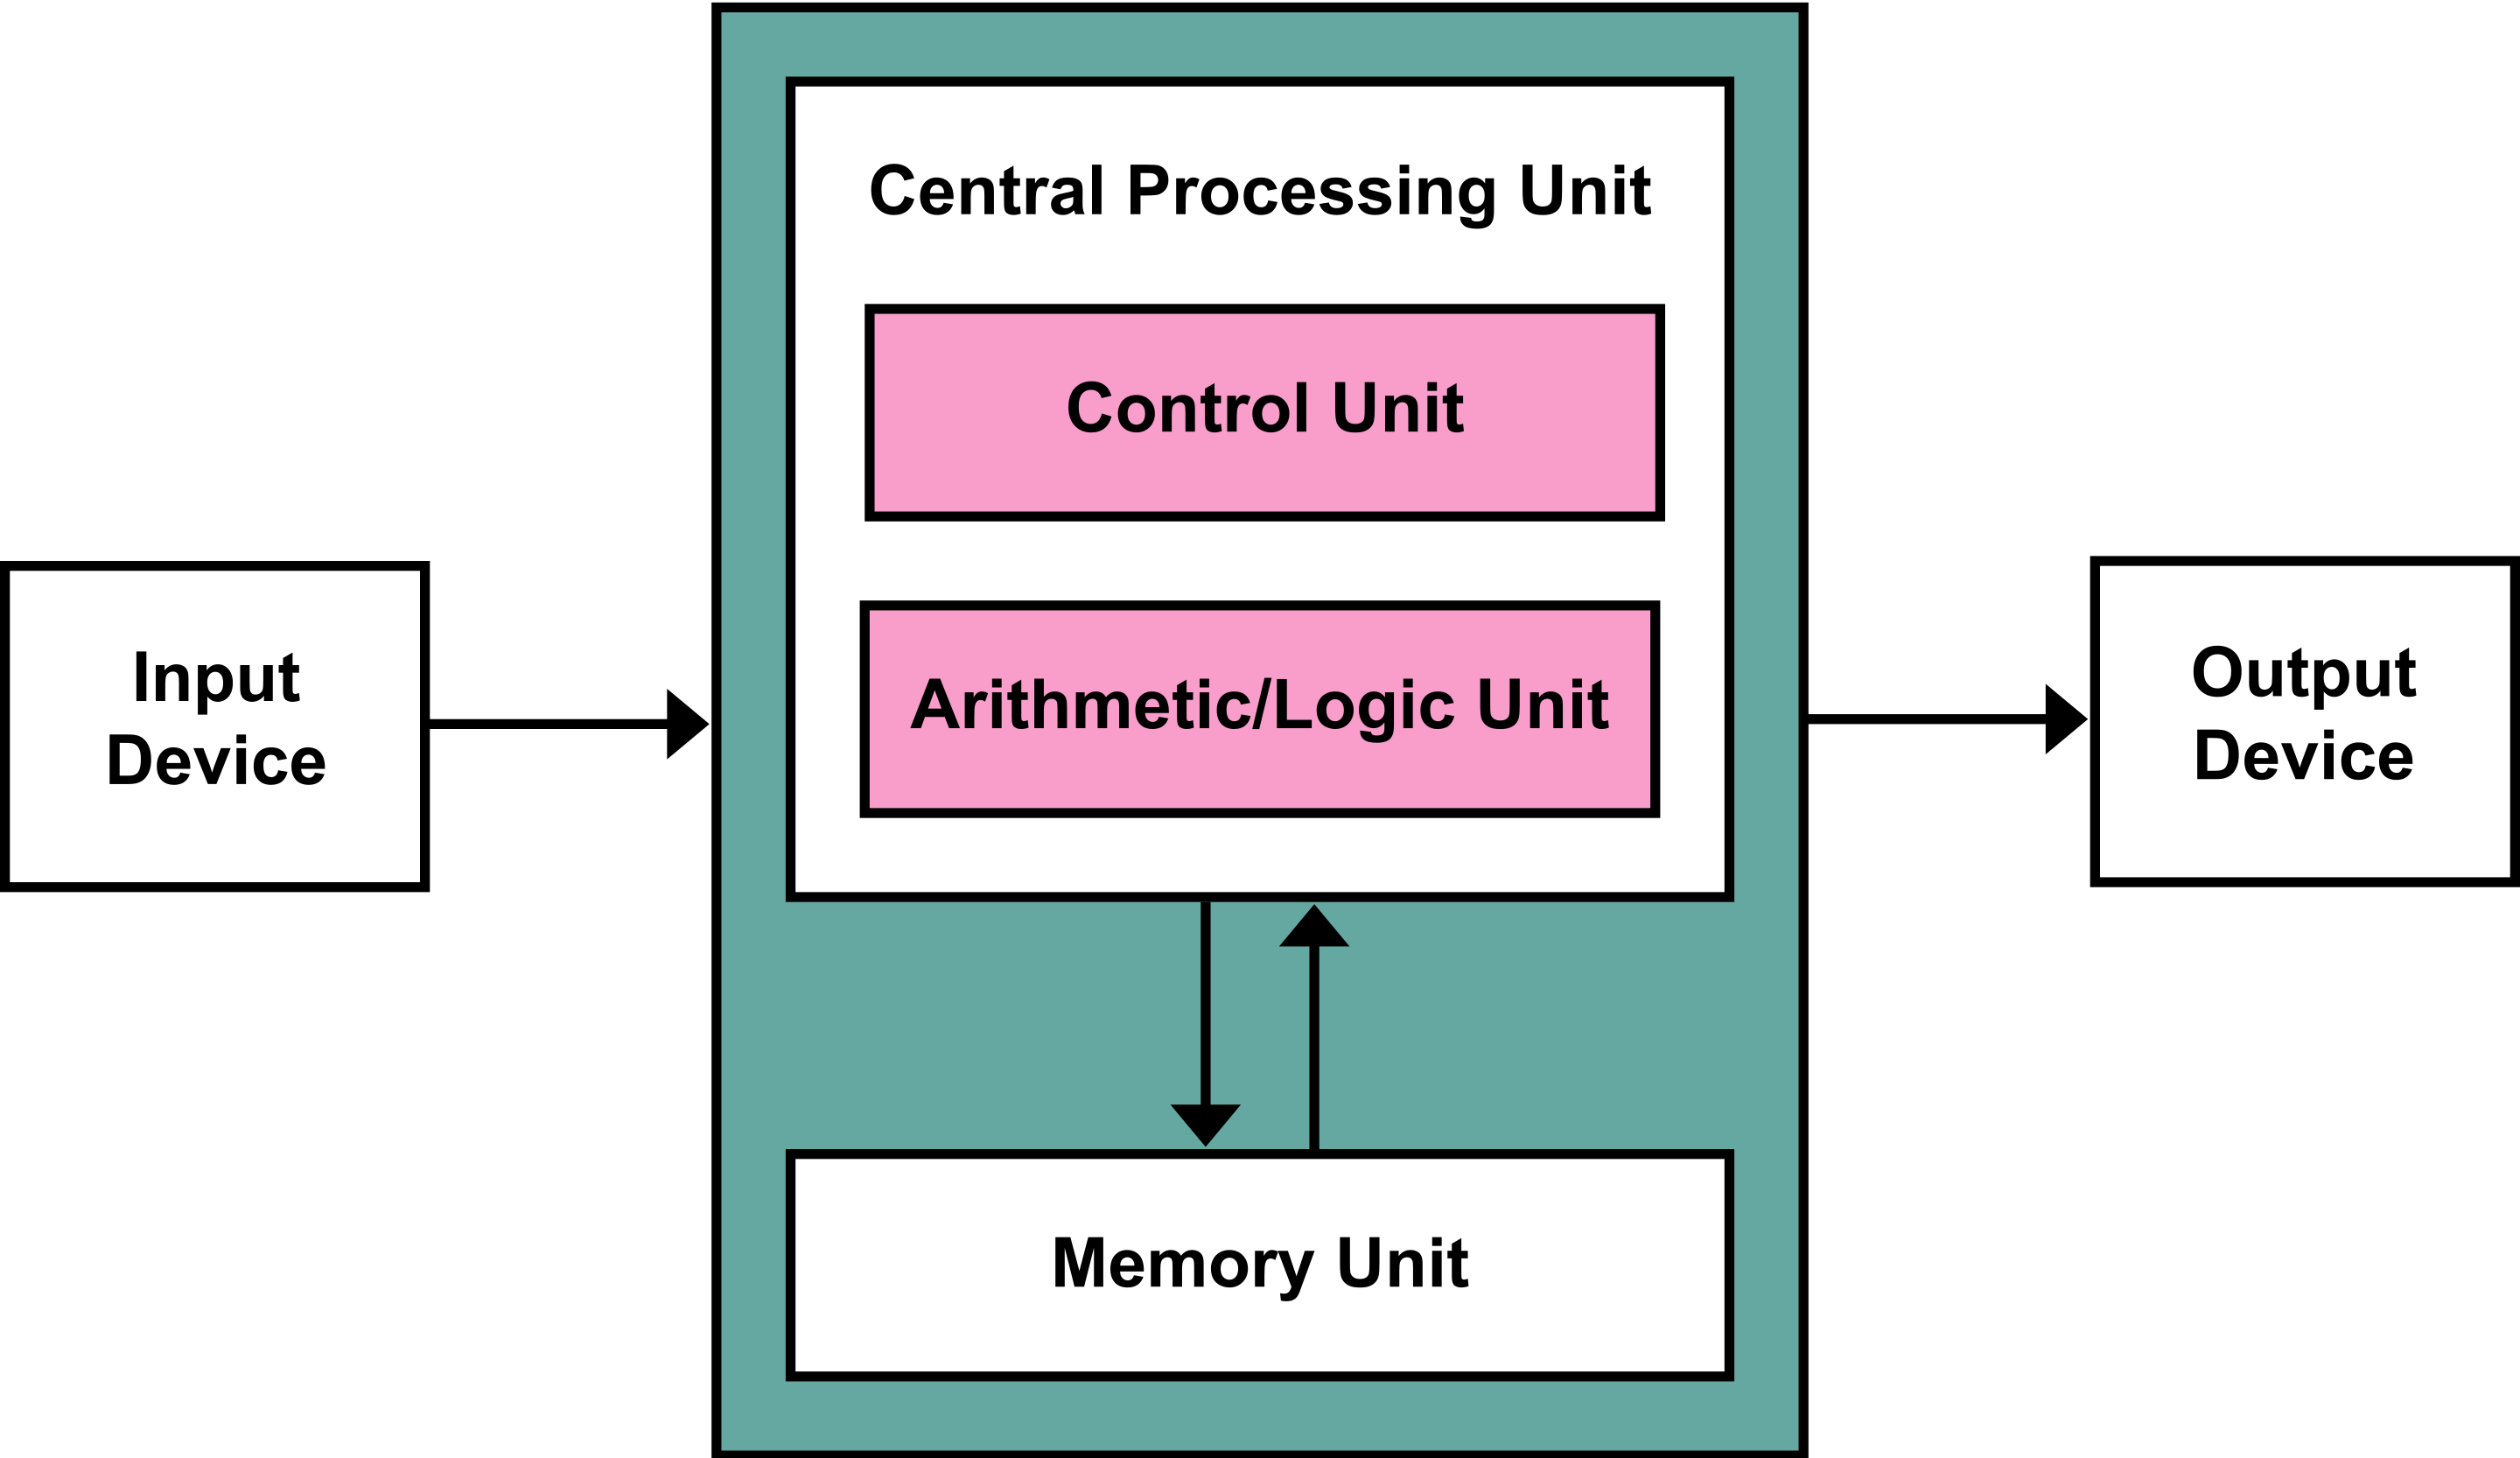
\includegraphics[width=0.8\textwidth]{von_neumann_architecture.png}}
  \caption{\label{von_neumann_architecture} Diagrama arquitetura de Von Neumann} 
\end{figure}

Nessa arquitetura, o cabeçote passa a ser uma CPU (Central Processing Unit), a fita se transforma em memória RAM e as operações são construídas e executadas em circuitos formados por portas lógicas chamadas de ULA (unidade lógica e aritmética) \cite{12}.

Atualmente, a maioria dos computadores modernos são construídos sobre a práxis da arquitetura von Neumann. A fim de simular um processador moderno de forma didática, foi elaborado o emulador \href{https://gzsig.io/vm-24bits/}{ASM 24bits} que permite a sua programação utilizando um Assembly\footnote{Uma linguagem assembly é uma linguagem de programação de baixo nível projetada para um tipo específico de processador. Ele pode ser produzido compilando o código-fonte de uma linguagem de programação de alto nível (como C / C ++), mas também pode ser escrito do zero.} de 20 instruções. Similar à arquitetura de von Neumann esse emulador é composto por memória e CPU, na qual a última possui dois registradores descritos abaixo:

\vspace{1cm}
\begin{longtable}{ |p{3cm}||p{11cm}|  }
  \hline
  \multicolumn{2}{|c|}{Registradores} \\
  \hline
    Nome &
    Descrição\\
  \hline
    Accumulator (ACC) &
    Registro mais usado para armazenar dados extraídos da memória. Está em diferentes números em diferentes microprocessadores. \\
  \hline
    Instruction Register (IR) &
    Registro que contém a instrução que está sendo executada no momento. \\
  \hline
  \caption{Registradores ASM 24 bit}
  \label{registers_asm}
\end{longtable}
\vspace{1cm}

Dentro da CPU, está a unidade lógica aritmética (ULA), um circuito digital usado para realizar operações aritméticas e lógicas. Ela representa o bloco de construção fundamental da unidade central de processamento (CPU). No caso do ASM 24bits, a sua ULA possui 20 instruções, sendo elas:

\vspace{1cm}
\begin{longtable}{ |p{3cm}||p{11cm}|  }
  \hline
  \multicolumn{2}{|c|}{ULA} \\
  \hline
  Mnemônico &
  Descrição\\
  \hline
  nop &
  Slot de memória vazio \\
  \hline
  jmp &
  Salto incondicional. Recebe uma variável como parâmetro e executará o código a partir da linha abaixo. \\
  \hline
  jz &
  Salta se o valor do acumulador (AC) é 0. Recebe uma variável como parâmetro e executa o código a partir da linha abaixo se o valor do AC for zero. Se o valor de AC NÃO for zero, a próxima linha será executada. \\
  \hline
  jnz &
  Pula se o valor do acumulador (AC) NÃO é 0. Recebe uma variável como parâmetro e executa o código a partir da linha abaixo se o valor do AC não for zero. Se o valor de AC for zero, a próxima linha será executada. \\
  \hline
  lv &
  Carrega uma constante diretamente no acumulador. Recebe uma constante em notação hexadecimal 0x00F2 por exemplo. \\
  \hline
  add &
  Adiciona uma constante ao valor do acumulador. Recebe uma constante em notação hexadecimal 0x00FA por exemplo. \\
  \hline
  addm &
  Recebe uma variável como parâmetro e adiciona o valor da variável ao valor do acumulador. \\
  \hline
  sub &
  Subtrai uma constante do valor do acumulador. Recebe uma constante em notação hexadecimal 0x00FA por exemplo. \\
  \hline
  subm &
  Recebe uma variável como parâmetro e subtrai o valor da variável do valor do acumulador. \\
  \hline
  mul &
  Multiplica uma constante do valor do acumulador. Recebe uma constante em notação hexadecimal 0x00FA por exemplo. \\
  \hline
  mulm &
  Recebe uma variável como parâmetro e multiplica o valor da variável pelo valor do acumulador. \\
  \hline
  div &
  Divide o valor do acumulador por uma constante. Recebe uma constante em notação hexadecimal como parâmetro, 0x00FA por exemplo. \\
  \hline
  divm &
  Recebe uma variável como parâmetro e divide o valor do acumulador pelo valor da variável. \\
  \hline
  load &
  Recebe uma variável como parâmetro e carrega o valor da variável para o acumulador. \\
  \hline
  stor &
  Armazena o valor atual do acumulador em uma variável. \\
  \hline
  sc &
  Chamada de função. \\
  \hline
  rc &
  Retorno de função, irá pular para a linha abaixo da chamada de função mantendo o valor atual no acumulador. \\
  \hline
  end &
  Irá parar a execução do programa. \\
  \hline
  in &
  Solicita ao usuário uma entrada (o número inserido deve ser em hexadecimal) e carrega a entrada no acumulador. \\
  \hline
  out &
  Alerta o usuário com o valor atual do acumulador. \\
  \hline
  \caption{Instruções ASM 24 bit}
  \label{table:2}
\end{longtable}
\vspace{1cm}

É a partir das instruções pertencentes à ULA que se compõem uma  Linguagem Assembly, essencial para o funcionamento de qualquer computador clássico e utilizada na criação do ASM 24bits (mencionado acima). A linguagem Assembly, frequentemente abreviada como ``asm'', é uma linguagem de programação de baixo nível em que há uma correspondência muito forte entre as instruções da linguagem e as instruções do código de máquina\footnote{Na programação de computadores, o código de máquina, que consiste em instruções em linguagem de máquina, é uma linguagem de programação de baixo nível usada para controlar diretamente uma CPU. Cada instrução faz com que a CPU execute uma tarefa muito específica, como uma carga, um armazenamento, um salto ou uma operação ALU em uma ou mais unidades de dados nos registros ou memória da CPU.}, sendo altamente dependente do hardware que está sendo utilizado. Dessa forma, a asm é indispensável durante a primeira etapa do `boot', já que o hardware ainda não está configurado para o sistema operacional. 

Assim, ao ligar qualquer computador clássico da atualidade, ele passará por algumas etapas importantes antes de poder ser utilizado por seu usuário final. Ao reiniciarmos um computador ele deverá carregar o sistema operacional de qualquer variante (Mac, Windows, Linux, etc.), a partir de algum dispositivo de armazenamento permanente que está atualmente conectado ao computador: seja um cd, um disco rígido, um USB, etc. O ambiente pré-SO oferece poucos serviços de alto nível. Neste estágio, mesmo um sistema de arquivos simples, que possa ler e gravar arquivos lógicos em um disco, seria um luxo. Felizmente, temos disponível o Basic Input/Output Software (BIOS), uma coleção de rotinas de software que são carregadas inicialmente de um chip para a memória e inicializadas quando o computador é ligado. O BIOS fornece detecção automática e controle básico dos dispositivos essenciais do seu computador, como tela, teclado e discos rígidos. Depois que este conclui alguns testes de baixo nível do hardware, principalmente se a memória instalada está funcionando corretamente ou não, ele deve iniciar o sistema operacional já armazenado em um de seus dispositivos. No entanto, precisamos lembrar que o BIOS não pode simplesmente carregar um arquivo que represente seu sistema operacional a partir de um disco, pois o ele não tem noção de um sistema de arquivos. Este deve ler setores específicos de dados (geralmente 512 bytes de tamanho) de localizações físicas específicas dos dispositivos de disco, para carregar do sistema operacional.

É a partir desses conceitos abordados que se constitui a estrutura básica da computação clássica, que dependem da física clássica para operar. Estes são os computadores tradicionais que usamos em nosso dia-a-dia – sejam eles Apple, Samsung, Dell ou qualquer outro –, também classificados como computadores binários, pois processam as instruções a partir de números binários, compostos apenas pelos símbolos ``1'' e ``0'', ligado e desligado, respectivamente. Assim, julga-se importante e de larga relevância ao tema compreender essa representação numérica.

Números binários ou números em base 2 são compostos por apenas dois dígitos, \{0, 1\}. Dessa forma, seu funcionamento é similar ao sistema decimal, ou base 10, que são compostos por dez dígitos, \{0; 9\}. No sistema decimal, é simples contar até nove, porém não existe um símbolo ou dígito para representar o número dez, sendo então representado por dois dígitos, ``10'', sendo uma simples lógica de posicionamento. Mais uma vez, após o número ``99'', é necessário utilizar da mesma regra para representar o número cem, ``100''. Já em base 2, o número zero é representado pelo símbolo ``0'', e o número um por ``1''. O mesmo dilema é enfrentado ao chegar no próximo valor: dois. E então é usada a mesma lógica de posicionamento, em base dois. Desta forma, o número dois é representado por ``10'', o três por ``11'', quatro por ``100'' e assim por diante. Portanto, números binários podem se tornar longos e compostos por muitos dígitos que levam o nome de bits \cite{6}. É com base nos \label{bits}bits\footnote{A menor unidade de informação que pode ser armazenada ou transmitida na comunicação de dados.} ligados e desligados que o computador baseia a sua linguagem. Para transforma-lo em base dez é preciso avaliar o valor de cada bit de acordo com a sua posição. 

Exemplo: número binário $1011$:

\[ 1011(b) = 1*2^3 + 0*2^2 + 1*2^1 + 1*2^0\]
\[ = 8 + 0 + 2 + 1 = 11(decimal)\]

O peso de cada bit de um número binário depende da sua posição relativa ao número completo, sempre partindo da direita para a esquerda.

\begin{itemize}
  \item O peso do primeiro bit é $bit * 2^0$
  \item O peso do segundo bit é $bit * 2^1$
  \item O peso do terceiro bit é $bit * 2^2$
  \item O peso do quarto bit é $bit * 2^3$
\end{itemize}

A fórmula ilustrada acima, pode ser exemplificada em uma fórmula genérica: 

\[= nth\: bit * 2^{n-1}\]

É possível notar que a regra para números binários, se repete para números em base 10.

Exemplo: número decimal $4392$:
\begin{itemize}
  \item O peso do primeiro bit é $2 * 10^0$
  \item O peso do segundo bit é $9 * 10^1$
  \item O peso do terceiro bit é $3 * 10^2$
  \item O peso do quarto bit é $4 * 10^3$
\end{itemize}
\[ 4392 = 4*10^3 + 3*10^2 + 9*10^1 + 2*10^0\]
\[= nth\: bit * 10^{n-1}\]

Essa regra se mantém verdadeira para qualquer base numérica.

\[= nth\: bit * (base)^{n-1}\]






Apesar dos computadores funcionarem a partir de números binários, ao se referir a eles é comum se usar notação hexadecimal. No entanto, pode-se questionar o porquê desse uso, já que é mais natural que optemos por usar os números em base 10, uma vez que culturalmente estamos mais acostumados a eles. Georges Ifrah em seu livro, ``The Universal History of Numbers'' \cite{14} aponta que:

``Traços da origem antropomórfica dos sistemas de contagem podem ser encontrados em muitas línguas. Na língua Ali (África Central), por exemplo, ``cinco'' e ``dez'' são respectivamente moro e mbouna: moro é na verdade a palavra para ``mão'' e mbouna é uma contração de moro (``cinco'') e bouna, que significa ``dois'' (portanto, ``dez'' = ``duas mãos'').

Portanto, é muito provável que as palavras indo-européias, semíticas e mongóis para os dez primeiros números derivem de expressões relacionadas à contagem dos dedos.''

Nesse sentido, Ifrah explica que:

``[...] a mão torna os dois aspectos complementares dos inteiros inteiramente intuitivos. Ele serve como um instrumento que permite o movimento natural entre a numeração cardinal e ordinal. Se você precisa mostrar que um conjunto contém três, quatro, sete ou dez elementos, você levanta ou dobra simultaneamente três, quatro, sete ou dez dedos, usando sua mão como mapeamento cardinal. Se quiser contar as mesmas coisas, dobre ou levante três, quatro, sete ou dez dedos em sucessão, usando a mão como ferramenta de contagem ordinal.''

Partindo dessa explicação, surge a ideia de números sendo representados a partir de 10 símbolos distintos: \{0; 9\}. Assim, o número decimal tem uma base de dez (ou seja, dez símbolos de dígitos distintos), já o número hexadecimal tem uma base de 16, por tanto, sendo necessário criar seis novos símbolos numéricos para possibilitar a contagem de 0 a 15 com apenas um símbolo. A maneira mais simples é usando algumas letras, como: 0,1,2, ... 8,9, a, b, c, d, e, f, em que, por exemplo, o símbolo `d', representaria uma contagem de 13.

Para distinguir entre hexadecimal e outros sistemas numéricos, costumamos usar o prefixo ``$0x$'', que é especialmente importante para indicar dígitos hexadecimais que podem não conter nenhum dos dígitos da letra, por exemplo: $0x50$ não é igual $(decimal) 50$ – $0x50$ é realmente $(decimal) 80$.

A questão é que um computador representa um número como uma sequência de bits, uma vez que fundamentalmente seu circuito pode distinguir apenas entre dois estados elétricos: 0 e 1 – fazendo referência ao motivo pelo qual usamos base 10, é como se o computador tivesse um total de apenas dois dedos. Portanto, para representar um número maior que 1, o computador pode agrupar uma série de bits, assim como podemos contar para além de 9 agrupando dois ou mais símbolos, por exemplo, 456, 23, etc.

Para facilitar a conversa sobre o tamanho dos números com os quais estamos lidando foram adotadas nomenclaturas para séries de bits de certos comprimentos. As instruções da maioria dos computadores lidam com um mínimo de valores de 8 bits, que são denominados bytes. Outros agrupamentos são ``short'', ``int'' e ``long'', que geralmente representam valores de 16 bits, 32 bits e 64 bits, respectivamente. Também tem-se o termo ``word'', que é usado para descrever o tamanho da unidade máxima de processamento do modo atual da CPU: portanto, no modo real de 16 bits, a ``word'' se refere a um valor de 16 bits, já no modo protegido de 32 bits, uma ``word'' se refere a um valor de 32 bits e assim por diante.

Desse modo, devido as sequências de bits serem compridas é mais fácil converte-las para notação hexadecimal do que para o sistema decimal natural, ilustrado na imagem abaixo. Assim, é possível quebrar a conversão em segmentos menores de 4 bits do número binário, em vez de tentar somar todos os bits componentes em um total geral, o que seria muito mais difícil para cadeias de bits maiores, como para: 16, 32, 64, etc. 

\vspace{1cm}
\begin{figure}[H] \centering 
  \makebox[\textwidth][c]{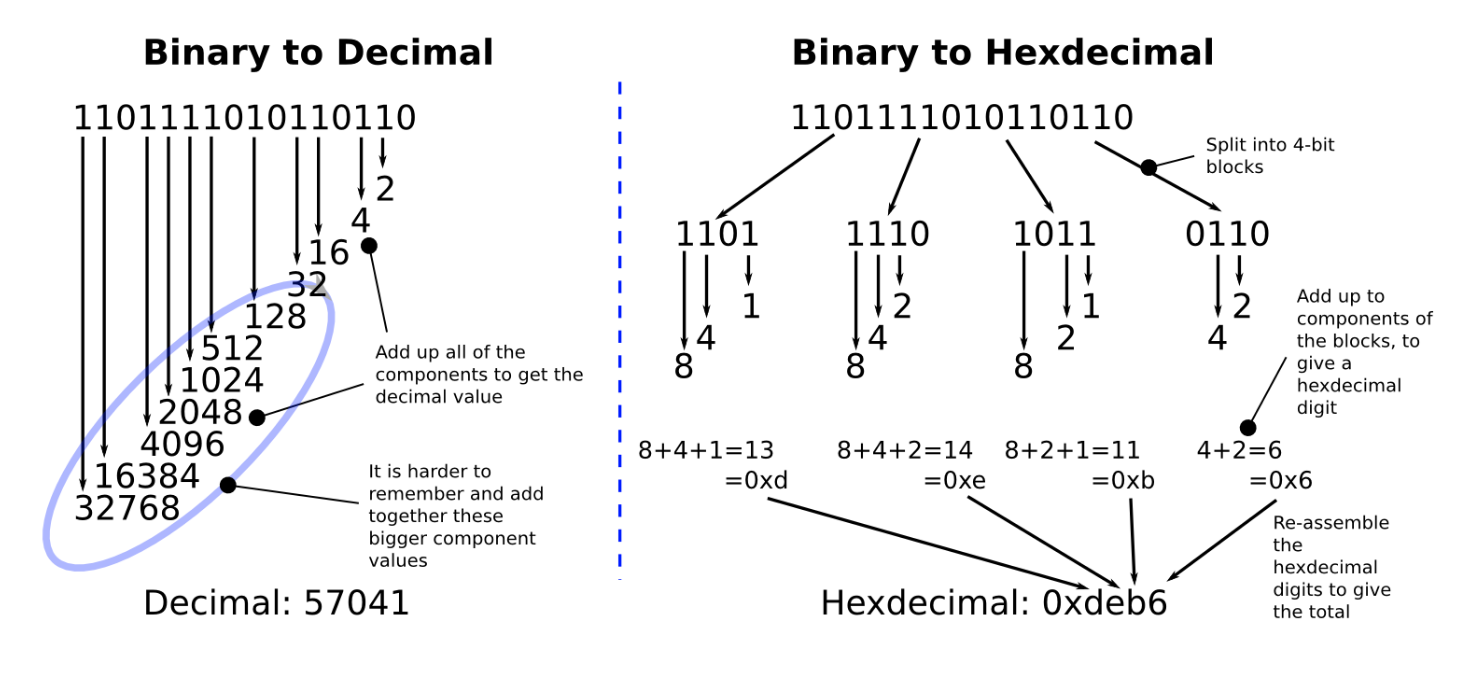
\includegraphics[width=0.8\textwidth]{binary_conversions}}
  \caption{\label{fig:4} Conversão de 1101111010110110 para decimal e hexadecimal} 
\end{figure}

Esse capítulo constituiu-se em apresentar conteúdos básicos e essenciais para possibilitar a compreensão do funcionamento de computadores clássicos. Conteúdos que foram compreendidos a partir do desenvolvimento de um \href{https://github.com/gzsig/zsig-OS}{sistema operacional} simples que passa por todas as etapas essenciais do processo de ``boot'' do \textit{state-of-art} de computadores clássicos: ligando em `modo real de 16 bits', transferindo-se para `modo protegido de 32 bits' e `gerenciando interrupções'.

Uma vez que o conteúdo sobre a computação clássica foi absorvido, podemos avançar para a próxima geração: computadores quânticos.
\newpage
